\begin{figure*}
  \centering
  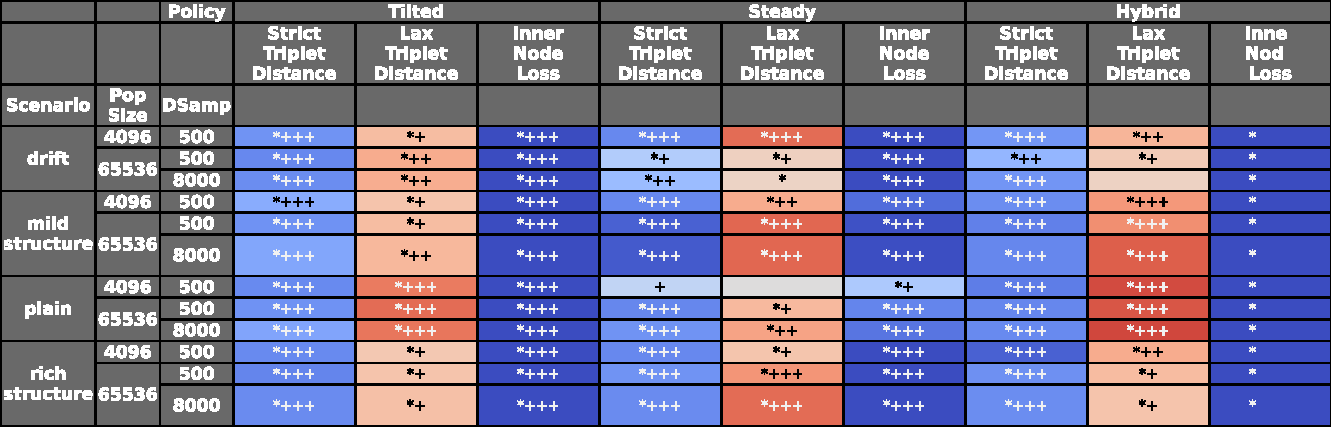
\includegraphics[width=\textwidth]{binder/binder/bit-vs-byte/outplots/bit-vs-byte-table}
  \caption{%
   \textbf{Comparison of reconstruction quality from bit- and bite-width differentiae.}
   \footnotesize
    Color coding reflects non-parametric comparison between quality measure values, with red indicating superior byte-width differentia performance and blue indicating superior bit-width differentia performance.
    In cell annotations, +'s indicatve small, medium, and large effect sizes using the Cliff's delta statistic and *'s indicate statistical significance at $\alpha = 0.05$ via Mann-Whitney U test.
  }
  \label{fig:bit-vs-byte}
\end{figure*}
